% \documentclass[12pt]{article}
\documentclass[12pt]{ctexart}
\usepackage[utf8]{inputenc}

\usepackage[english]{babel}
\usepackage[dvips]{epsfig}
\usepackage{amsmath}
\usepackage{amssymb}
\usepackage{amsfonts}
\usepackage{amsthm}
\usepackage{amsbsy}
\usepackage{amsgen}
\usepackage{amscd}
\usepackage{amsopn}
\usepackage{amstext}
\usepackage{amsxtra}
\usepackage{mathrsfs}
\usepackage{enumitem}
\usepackage{graphicx}
\usepackage{verbatim}
\usepackage{epstopdf}
\usepackage{float}
\usepackage[all,cmtip]{xy}
\usepackage{accents}
\usepackage{sseq}
\usepackage{url}
\usepackage{hyperref}
\usepackage{makeidx}
\usepackage{siunitx}
\usepackage{xcolor}
\usepackage{physics}

%%%%%%%%% 版面设置 %%%%%%%%%%%%%%%%%%%%%%%%%%%%%%%%%%%%%%
\usepackage{geometry}
\usepackage{titlesec}
\usepackage{fancyhdr}\pagestyle{empty}
\titleformat*{\section}{\large\bfseries}

%
\geometry{
	a4paper,
	total={170mm,240mm},
	left=20mm,
	top=30mm,
}

%Bitte nicht einstellen
\renewcommand{\figurename}{Abbildung}
\renewcommand{\tablename}{Tabelle}
\pagestyle{fancyplain}
\headheight 35pt
\lhead{\name}
\chead{\textbf{\Large \Title}}
\rhead{\due\\\today}
\lfoot{}
\cfoot{}
\rfoot{\small\thepage}
\headsep 1.5em

%%%%%%%%%%%%%%%%%%%%%%%%%%%%%%%%%%%%%%%%%%%%%%%%%%%%%%

\newtheorem{thm}{Theorem}[section]

% 定义解题环境
\theoremstyle{remark}
\newtheorem{remark}[thm]{Remark}
\newtheorem{theorem}{Theorem}
\newtheorem{observation}[thm]{Observation}

\theoremstyle{definition}
\newtheorem{problem}{\text{}}
\newtheorem{Problem}{\text{Problem}}
\newtheorem*{solution}{解}
\newtheorem*{Answer}{Answer}
\newtheorem{example}{Example} 

%%%%%%%%%%%%%%%%%%%%%%%%%%%%%%%%%%%%%%%%%%%%%%%%%%%%%%%%%%%%%%%%%%
\newcommand\name{陈景龙22120307}
\newcommand\due{-}
\newcommand{\emptyline}{\vspace{0.6\baselineskip}}

\newcommand\Title{2021智能计算数学基础试卷}
\renewcommand\due{due: November 6, 2022}
\newcommand\minimize{\operatorname{minimize}} % 最小化
\newcommand\maximize{\operatorname{maximize}} % 最大化
\newcommand\subject{\operatorname{subject\ to}}

\newcommand{\todo}{{\color{red} to do}} % to do

\begin{document}

% \maketitle

\begin{problem}
	计算向量$(1,-1,2,3)$的$l_1$范数。
	\solution $$\|(1,-1,2,3)\|_1=\sum_{i=1}^n|x_i|=1+1+2+3=7$$
\end{problem}

\begin{problem}
	计算函数极限:$\lim_{x\to \infty}(1+\frac{1}{2x})^{6x}$
	\solution \begin{align*}
		&\lim_{x\to \infty}(1+\frac{1}{2x})^{6x}\\
		=&\lim_{x\to \infty}(1+\frac{1}{2x})^{2x\cdot 3}\\
		=&e^3
	\end{align*}
\end{problem}


\begin{problem}
	判断题:级数$\sum_{n\ge 1}\frac{n^2+n+1}{n^3+n^2+n+1}$收敛。
	\solution 否。
\end{problem}

\begin{problem}
	判断题:集合$\left\{(x,y)\in\mathbb{R}^{2}:x^2+2y^2<1,x+y<1\right\}$是开集。
	\solution 是。
\end{problem}

\begin{problem}
	计算函数$f(x,y)=\frac{x}{x^2+y^2}$在$(0,1)$点处的梯度。
	\solution$\nabla f(a)=(\partial_xf,\partial_yf)^t$,而$\partial_xf=\frac{y^2-x^2}{(x^2+y^2)^2},\partial_yf=-\frac{2xy}{x^2+y^2}$。所以$\nabla f(0, 1)=\left(1, 0\right)^t$。
\end{problem}


\begin{problem}
	计算函数$f(x,y)=x^2+2xy+3y^2+4y$的极小值。
	\solution \[\begin{cases}
		\nabla f_x = 2x + 2y = 0\\
		\nabla f_y = 2x + 6y + 4 = 0
	\end{cases}\]
	可得 $(x, y) = (1, -1)$,
	\[\nabla^2f = \begin{pmatrix}
		2 & 2\\
		2 & 6
	\end{pmatrix}\] 
	$\nabla^2f$ 是一个正定矩阵,所以 $(x, y) = (1, -1)$ 是极小值点,$f(1, -1) = -2$。
\end{problem}

\begin{problem}
	给出二次函数$f(x)=\frac{1}{2}x^tPx+q^tx+r$的极小值点,其中$P\in\mathbb{S}_{++}^n,q\in\mathbb{R}^n,r\in\mathbb{R}$。
	\solution \begin{align*}
		f(x + \varepsilon) - f(x) =& \frac{1}{2} (x + \varepsilon)^tP(x + \varepsilon) + q^t(x + \varepsilon) + q \\
		& -\frac{1}{2} x^tPx - q^tx - r\\
		=& \frac{1}{2}x^tP\varepsilon + \frac{1}{2}\varepsilon^tPx + q^t\varepsilon + \frac{1}{2}\varepsilon^tP\varepsilon\\
		=& (x^tP + q^t)\varepsilon + \frac{1}{2}\varepsilon^tP\varepsilon
	\end{align*}
	
	由 $f(x + \varepsilon) = f(x) + \nabla f(x)^t\varepsilon + \frac{1}{2}\varepsilon^t \nabla^2 f(x) \varepsilon + o(\|\varepsilon\|^2)$ 可得,$\nabla f(x) = Px + q, \nabla^2 f(x) = P$。
	
	并且 $\nabla^2 f(x) = P\in \mathbb{S}^n_{++}$,所以 $\nabla f(x^*) = 0$,$x^*$ 即为极小值点,极小值点 $x^* = -P^{-1}q$。
\end{problem}


\begin{problem}
	给定$P\in\mathbb{S}_{++}^n$以及约束条件$\|x\|\le 1$,二次函数$f(x)=x^tPx$的极大值是多少?
	\solution $P = U^tVU$,则 $f(x) = x^tU^tVUx$,$y = Ux$,则原问题变为 $f(y) = y^tVy = \sum y_i^2v_i$,约束条件 $\norm{y}^2 \le 1$,即 $\sum y_i^2 \le 1$。所以 $f(x)$ 最大值为矩阵 $A$ 的最大特征值 $\max(v_i)$,其中 $v_i$ 表示矩阵 $A$ 的第 $i$ 个特征值。
\end{problem}

\begin{problem}
	求出下述优化问题的极小值\[\begin{cases}
		\minimize\quad & f(x, y, z)=3 x^{2}+3 y^{2}-z^{2}+x y+x z \\
		\subject\quad & x+y+z=1
	\end{cases}\]
	\solution \begin{gather*}
		L(x, y, z, \mu) = 3x^2 + 3y^2 - z^2 + xy + xz + \mu(x + y + z - 1)\\
		\partial_xL = \partial_yL = \partial_zL = 0\\
		\begin{cases}
			x + y + z - 1 &= 0\\
			6x + y + z + \mu &= 0\\
			6y + x + \mu &= 0\\
			-2z + x + \mu &= 0
		\end{cases}
	\end{gather*}
	
	解得 $(x, y, z, \mu) = (-4, -\frac{5}{2}, \frac{15}{2}, 19)$。

	$$\nabla^2 f = \begin{pmatrix}
		6 & 1 & 1 \\
		1 & 6 & 0 \\
		1 & 0 & -2
	\end{pmatrix}$$

	$$B = (\alpha_1, \alpha_2) = \begin{pmatrix}
		1 & 1 \\
		-1 & 0 \\ 
		0 & -1
	\end{pmatrix}$$

	$$B^t\nabla f B = \begin{pmatrix}
		 10 & 4 \\ 
		 4 & 2 \\
	\end{pmatrix}$$
	$B^t\nabla f B$ 是一个正定矩阵,所以 $f_{min} = f(-4, -\frac{5}{2}, \frac{15}{2}) =  -\frac{19}{2}$
\end{problem}

\begin{problem}
	设$f(A)=\|X-AY\|^2$,其中$A,X$和$Y$分别是维度为$n\times m,n\times k,m\times k$的矩阵,计算$Df(A)$。
	\solution \begin{align*}
		f(A) =& \|X - AY\|^2 \\
		=& \tr\left((X - AY)(X - AY)^t\right) \\
		=& \tr\left(XX^t - XY^tA^t - AYX^t + AYY^tA^t\right)
	\end{align*}
	由 $f(A) = \tr(ABA^t) \Longrightarrow Df(A) = A(B + B^t), f(A) = \tr(AB) \Longrightarrow Df(A) = B^t$,可得 \[Df(A) = 2AYY^t - 2XY^t\]
\end{problem}

\begin{problem}
	判断题:$\rank(A^tA)=\rank(A)$。
	\solution 是。\begin{itemize}
		\item $x \in \mathcal{N}(A) \Longleftrightarrow A x=0 \Longrightarrow A^{T} A x=0 \Longleftrightarrow x \in \mathcal{N}(A^TA)$
		\item $x \in \mathcal{N}(A^TA) \Longleftrightarrow A^{T} A x=0 \Longrightarrow A x \in \mathcal{N}\left(A^{T}\right) \Longrightarrow A x \in \mathcal{N}\left(A^{T}\right) \bigcap C(A)=\{0\} \Longleftrightarrow x \in \mathcal{N}(A)$
	\end{itemize}
	所以 $\mathcal{N}(A) = \mathcal{N}(A^tA) = n - r$,$\rank(A^tA) = \rank(A) = r$。
\end{problem}

\begin{problem}
	判断题:设$A,B$为列数相同的矩阵,$C=\begin{pmatrix}A\\B\end{pmatrix}$,则他们的零空间满足:$\mathcal{N}(C)=\mathcal{N}(A)\cup \mathcal{N}(B)$。
	\solution 否。矩阵的秩可能变大,那么零空间维度可能变小。$\mathcal{N}(C) = \mathcal{N}(A)\cap \mathcal{N}(B)$.
\end{problem}

\begin{problem}
	判断题:如果$u,v$是单位向量,则$u+v$和$u-v$是正交的。
	\solution 是。$(u + v)^t(u - v) = u^tu - u^tv + v^tu - v^tv = 0$。
\end{problem}

\begin{problem}
	判断题:设$A,B$是$n$阶方阵,则$AB$和$BA$具有相同的特征值。
	\solution 是。若 $ABx = \lambda x(\lambda \neq 0)$,则有 $Bx \neq x$,且 $BA(Bx) = B\lambda x = \lambda (Bx)$,都有相同的特征值 $\lambda$。特征向量分别是 $x$ 和 $Bx$.
\end{problem}

\begin{problem}
	判断题:设$x$是$A^tA$的特征值不为$0$的特征向量,则$Ax$是$AA^t$的特征向量。
	\solution 是。$A^tAx = \lambda\boldsymbol{x} \Longrightarrow AA^t(A\boldsymbol{x}) = \lambda (A\boldsymbol{x})$,$A\boldsymbol{x}$是$AA^t$的特征向量。
\end{problem}

\begin{problem}
	将向量$(2,1)$以向量$(1,2)$为轴做对称,得到的向量是什么?
	\solution 两倍的投影向量减原向量
	\begin{align*}
		u &= (2, 1)^t\\
		v &= (1, 2)^t\\
		u^\prime &= \frac{2vv^tu}{\|v\|^2} - u\\
		&=\left(-\frac{2}{5}, \frac{11}{5}\right)^t
	\end{align*}
\end{problem}

\begin{problem}
	计算矩阵$\begin{pmatrix}2&3\\1&2\end{pmatrix}$的奇异值。
	\solution \[A^TA = \begin{bmatrix}
		5 & 8 \\
		8 & 13
	\end{bmatrix}\]
	求特征值:\begin{align*}
		|\lambda I - A^TA| &= 0\\
		\begin{vmatrix}
			\lambda - 5 & -8 \\
			-8 & \lambda - 13
		\end{vmatrix} &= 0
	\end{align*}
	解得 $\lambda_1 = 9 + 4\sqrt{5}, \lambda_2 = 9 - 4\sqrt{5}$。即 $\sigma_1 = \sqrt{9 + 4\sqrt{5}}, \sigma_2 = \sqrt{9 - 4\sqrt{5}}$。化简得 $\sigma_1 = \sqrt{5} + 2, \sigma_2 = \sqrt{5} - 2$。
\end{problem}

\begin{problem}
	假设$n$阶方阵$A$有$n$个线性无关的特征向量,则随着$k\to \infty,A^k\to 0$的充分必要条件是什么?
	\solution $n$阶方阵$A$有$n$个线性无关的特征向量,则 $$\begin{aligned}
		A &= X\Lambda X^{-1} \\	
		A^k &= X \Lambda^k X^{-1}\\
		A^k &= X \begin{pmatrix}  
			\lambda_1^k &  &  \\  
			 & \ddots & \\  
			 &  & \lambda_n^k  
		\end{pmatrix} X^{-1} 
	\end{aligned}$$
	则随着$k\to \infty,A^k\to 0$的充分必要条件是 $\lambda_i < 1,\forall i\in [1, n]$。
\end{problem}

\begin{problem}
	假设$x_1\sim \mathcal{N}(0,\sigma^2),x_2\sim\mathcal{N}(0,\sigma^2)$,并且$x_1$和$x_2$独立,则$y=x_1^2+x_2^2$服从何种分布?
	\solution Chi-Squared 分布。
\end{problem}

\begin{problem}
	中心极限定理的“中心”是指什么?“极限”是指什么? 
	\solution 中心指高斯分布是所有分布的中心。极限指足够多的独立同分布之和趋近于高斯分布。
\end{problem}

\begin{problem}
	高斯白噪声中的“白”是什么意思?
	\solution 不同时刻的噪声正交。此时如果 $E(w(1)) = 0$ 或 $E(w(2)) = 0$,则 $w(1),w(2)$ 不相关,不相关的高斯噪声就是独立的高斯噪声。如果均值为 0 则不同时刻噪声相互独立。
\end{problem}

\begin{problem}
	假设随机变量$x$和$y$的联合概率密度为$f(x,y)=1/4$,其中$0\le x\le 2,1\le y\le 3$。请问$x$和$y$是否正交?是否独立?是否相关?
	\solution 不正交,独立,不相关。$f_X(x) = f_Y(y) = \frac{1}{2},f(x, y) = f_X(x)f_Y(y),0 \le x \le 2, 1 \le y \le 3$。
\end{problem}

\begin{problem}
	已知随机变量 $w=\sum_{i=1}^{500}z_i$ ,其中 $z_i$ 是相互独立的均匀分布随机变量,$z_i\sim\mathcal{U}(-\frac{\sqrt{3}}{10},\frac{\sqrt{3}}{10})$。 已知某一个测量数据 $y$ 和要估计的参数 $A$ 以及随机变量 $w$ 有线性关系:$y=4A+w$。请写出随机变量 $w$ 的近似概率密度函数。
	\solution $E(z_i) = 0, D(z_i) = \frac{1}{100}$。随机变量 $w$ 服从高斯分布 $\mathcal{N}(n\mu, n\sigma^2) = \mathcal{N}(0, 5)$。
\end{problem}

\begin{problem}
	条件如$23$题,写出似然函数$p(y|A)$的表达式,根据最大似然准则(ML)来获取$A$的估计值。
	\solution $p(y|A) \sim \mathcal{N}(4A, 5), p(y|A) = \frac{1}{\sqrt{10\pi}}e^{-\frac{(y - 4A)^2}{10}}$。
\end{problem}

\begin{problem}[\todo]
	条件如23题,利用最小二乘法(LS)来估计$A$,请给出表达式。
	\solution 
\end{problem}

\begin{problem}[\todo]
	条件如23题,假设$A$是高斯随机变量,$A\sim\mathcal{N}(0,1)$,且$A$和$w$相互独立。利用线性最小均方误差(LMMSE)准则来估计$A$,请给出表达式。
	\solution 
\end{problem}

\begin{problem}
	按照信息的性质,可以把信息分为哪三种基本类型?
	\solution 语法信息,语用信息,语义信息。
\end{problem}

\begin{problem}
	若一随机事件的概率为$p(x)$,写出它的自信息$I(x)$的数学定义。
	\solution $I(x) = -\log p(x)$ 
\end{problem}

\begin{problem}
	对于任意三个离散随机事件$x,y$与$z$,有$I(x;yz)=I(x;z)+I(x;y|z)$,这表明信息有何种性质?
	\solution 可加性.
\end{problem}

\begin{problem}
	已知两个信源分别为$\begin{pmatrix}X\\P\end{pmatrix}=\begin{pmatrix}a_1&a_2\\0.8&0.2\end{pmatrix}$和$\begin{pmatrix}Y\\Q\end{pmatrix}=\begin{pmatrix}b_1&b_2\\0.5&0.5\end{pmatrix}$则在信源熵$H(X)$和$H(Y)$中,较大的是哪一个,其值为多少bit/符号?
	\solution $H(Y) > H(X)$,等概分布信息熵最大\begin{itemize}
		\item $H(X) = -0.8\log_2 0.8 - 0.2\log_2 0.2 = \SI{0.702}{bit/\text{符号}}$
		\item $H(Y) = -0.5\log_2 0.5 - 0.5\log_2 0.5 = \SI{1}{bit/\text{符号}}$
	\end{itemize}
\end{problem}

\begin{problem}
	判断题:两个离散随机变量$X$与$Y$之间的平均互信息为$I(X;Y)=H(X)-H(Y\mid X)$。
	\solution 否。$I(X;Y)=H(X)-H(X\mid Y)$
\end{problem}

\begin{problem}
	判断题:对于固定的信源,平均互信息$I(X;Y)$具有凸状性,$I(X;Y)$是信道传递概率分布$P(Y/X)$的上凸函数。
	\solution 否。凸状性,$I(X; Y)$是二元函数:$P(X)$ 的上凸函数,$P(Y/X)$ 的下凸函数。
\end{problem}

\begin{problem}
	判断题:假设$p(x)$和$q(x)$是定义在同一概率空间上的两种概率测度,则$p$相对于$q$的信息散度定义为$D(p\|q)=\sum_xp(x)\log\frac{p(x)}{q(x)}$。
	\solution 是。
\end{problem}

\begin{problem}[\todo]
	遍历性马尔柯夫序列的极限熵为$H_\infty(X)=-\sum_{i,j}p_ip_{j,i}\log p_{j,i}$,其中序列间的相关性由公式中的哪个变量描述?
	\solution 
\end{problem}

\begin{problem}
	判断题:博弈问题中,一个纳什均衡解也是一个帕雷托最优解。
	\solution 否。纳什均衡解不一定是帕累托最优解,帕累托最优解不一定是纳什均衡解。
\end{problem}

\begin{problem}
	判断题:一个有限决策者且有限策略的博弈问题始终能找到至少一个纯策略纳什均衡解。
	\solution 否。比如猜拳游戏。
\end{problem}

\begin{problem}
	判断题:一个正则型博弈可以等价转化为一个不完美信息的扩展型博弈。
	\solution 是。两个人轮流操作,但是不知道对方怎么操作。
\end{problem}

\begin{problem}[\todo]
	判断题:扩展型博弈问题中,一个纳什均衡解也是一个子博弈精炼均衡解,而一个子博弈精炼均衡解未必是一个纳什均衡解。
	\solution 
\end{problem}

\begin{problem}
	判断题:不完全信息博弈中的不确定性比不完美信息博弈中的不确定性要高。
	\solution 是。不完全博弈不知道自己在进行什么博弈游戏,不完美博弈不知道自己处于哪个状态(博弈树的节点)。
\end{problem}

\begin{problem}[\todo]
	简要阐述需要利用逆向归纳法求解扩展型博弈(博弈树)的原因。
\end{problem}

\begin{figure}[htbp]
	\centering
	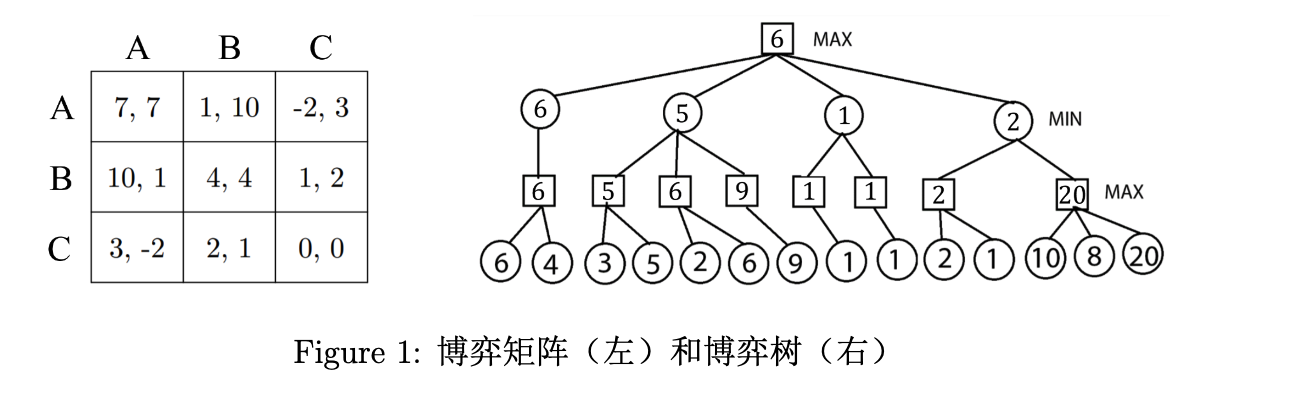
\includegraphics[width=1\textwidth]{./figure/fig1.png}
\end{figure}

\begin{problem}
	从图1左的博弈矩阵中,找出所有纯策略纳什均衡解,并简述判断理由。
	\solution $BB$,两个决策者在对方不改变策略的情况下,都已经处于最优解。
\end{problem}

\begin{problem}
	从图1右的博弈树中(MAX和MIN的minimax值己给出),找出可进行$\alpha-\beta$剪枝操作的三个位置。
	\solution $C-H,C-I,D-K,E-M$
\end{problem}

\begin{problem}
	判断题:NP-Complete问题的多项式时间复杂度算法都是近似算法。
	\solution 是.
\end{problem}

\begin{problem}
	设$X$是由有限元素构成的集合,$F$是由$X$的非空子集构成的集合且对于任意$X$中的元素$e$,都存在一个$F$中的元素$S$使得$e$是$S$中的元素,即$X=\cup_{S\in F}S$。考虑“集合覆盖问题”:求$F$中的一个子集$C\subseteq F$,使得$X=\cup_{S\in C}S$,且$C$的大小$|C|$最小。下面是证明“集合覆盖问题”是NP-complete的过程,请补充完善。首先请将“集合覆盖问题”转化为语言描述。
	\solution 集合覆盖问题:$\left\{\right.$ 存在由$X$的非空子集构成的集合 $F$ 的子集 $C$,$C \subseteq F$,子集 $C$ 的大小为 $|C|=k$,使得 $X=\cup_{S \in C} S$$\left.\right\}$。
\end{problem}

\begin{problem}
	接上题,请说明“验证集合覆盖问题”的时间复杂度是多项式时间复杂度。
	\solution 给定了集合 $C$,求集合 $C$ 的所有元素的并集,是多项式时间复杂度可解的。如果这个并集等于集合 $X$,那么这个问题为真。
\end{problem}

\begin{problem}
	顶点覆盖问题:$G=(V,E)$是无向图,$V$和$E$分别是顶点和边的集合,求$V$的子集$V^\prime$使得对于任意边$(u,v)\in E$都有$u\in V^\prime$或$v\in V^\prime$,且$V^\prime$的大小$|V^\prime|$最小。请将顶点覆盖问题转化为语言描述。
	\solution $\left\{<G, u, v, k>\right. : G = (V, E)$ 是一个无向图,存在一个大小为 $k$ 的顶点覆盖 $V^\prime$,使得 $E$ 中每一条边,都至少有一个点在 $V^\prime$ 中。 $\left.\right\}$
\end{problem}

\begin{problem}[\todo]
	已知顶点覆盖问题是NP-complete,请将该问题的实例转化为“集合覆盖问题”的实例。
	\solution
\end{problem}

\begin{problem}[\todo]
	接上题,说明转化过程是多项式时间复杂度的。
	\solution 
\end{problem}

\begin{problem}[\todo]
	利用上题结果,试证明:图$G=<V,E>$中存在大小为$k$的顶点覆盖当且仅当$<X,F>$中存在大小为$k$的集合覆盖。
	\solution 
\end{problem}

\end{document}